\documentclass[aspectratio=169]{beamer}
% Add slides directory to search path for Dartmouth theme
\makeatletter
\def\input@path{{../}}
\makeatother
\usetheme{Dartmouth}
\usepackage{graphicx}
\usepackage{tikz}
\usepackage{amsmath}
\usepackage{listings}
\usepackage{xcolor}
\usepackage{booktabs}
\usetikzlibrary{shapes,arrows,positioning,calc}

% Code listing setup
\lstset{
  basicstyle=\ttfamily\small,
  keywordstyle=\color{blue},
  commentstyle=\color{gray},
  stringstyle=\color{red},
  showstringspaces=false,
  breaklines=true,
  frame=single,
  language=Python
}

\title{Lecture 16: BERT Variants}
\subtitle{Week 6, Lecture 2 - Improvements and Optimizations}
\author{PSYC 51.07: Models of Language and Communication}
\date{Winter 2026}

\begin{document}

% ============================================================
% TITLE SLIDE
% ============================================================
\begin{frame}[shrink=10]
\titlepage
\end{frame}

% ============================================================
% OVERVIEW
% ============================================================
\begin{frame}[shrink=10]{Today's Agenda 📋}
\large
\begin{enumerate}\setlength{\itemsep}{0pt}
    \item 🚀 \textbf{RoBERTa}: Robustly Optimized BERT
    \item 🔬 \textbf{ALBERT}: A Lite BERT with parameter sharing
    \item ⚡ \textbf{DistilBERT}: Knowledge distillation for efficiency
    \item 🔌 \textbf{ELECTRA}: Replace Token Detection
    \item 📊 \textbf{Comparative Analysis}: When to use which variant
    \item 💻 \textbf{Practical Considerations}: Model selection guide
\end{enumerate}

\vspace{1em}
\textit{Goal: Understand improvements to BERT and choose the right model}
\end{frame}

% ============================================================
% BERT LIMITATIONS
% ============================================================
\begin{frame}[shrink=10]{BERT's Limitations ⚠️}
\textbf{What could be improved?}

\vspace{1em}

\begin{enumerate}\setlength{\itemsep}{0pt}
    \item \textbf{Training Procedure}
    \begin{itemize}\setlength{\itemsep}{0pt}
        \item Some choices seemed arbitrary
        \item NSP task might not be useful
        \item Static masking (same masks every epoch)
    \end{itemize}

    \vspace{0.5em}

    \item \textbf{Model Size}
    \begin{itemize}\setlength{\itemsep}{0pt}
        \item 110M (Base) or 340M (Large) parameters
        \item Large memory footprint
        \item Slow inference
    \end{itemize}

    \vspace{0.5em}

    \item \textbf{Training Efficiency}
    \begin{itemize}\setlength{\itemsep}{0pt}
        \item Only 15\% of tokens are predicted
        \item 85\% of computation "wasted"?
        \item Could we learn more efficiently?
    \end{itemize}

    \vspace{0.5em}

    \item \textbf{Data and Compute}
    \begin{itemize}\setlength{\itemsep}{0pt}
        \item Trained on limited data (3.3B words)
        \item Modern datasets much larger
        \item Could benefit from more training
    \end{itemize}
\end{enumerate}

\vspace{0.5em}
\textbf{Many variants address these issues!}
\end{frame}

% ============================================================
% ROBERTA
% ============================================================
\begin{frame}[shrink=10]{RoBERTa: Robustly Optimized BERT 🚀}
\textbf{Key idea: Better training = Better performance}

\vspace{1em}

\textbf{RoBERTa's Improvements (Liu et al. 2019):}

\begin{enumerate}\setlength{\itemsep}{0pt}
    \item \textbf{Remove NSP Task}
    \begin{itemize}\setlength{\itemsep}{0pt}
        \item Next Sentence Prediction hurt performance
        \item Use only Masked Language Modeling
        \item Full sentences (don't need sentence pairs)
    \end{itemize}

    \vspace{0.5em}

    \item \textbf{Dynamic Masking}
    \begin{itemize}\setlength{\itemsep}{0pt}
        \item Generate masking pattern every time
        \item BERT: static masks (same for every epoch)
        \item More diverse training signal
    \end{itemize}

    \vspace{0.5em}

    \item \textbf{Larger Batches, More Data}
    \begin{itemize}\setlength{\itemsep}{0pt}
        \item Batch size: 8K sequences (vs BERT's 256)
        \item 160GB text (vs BERT's 16GB)
        \item Longer training (500K steps vs 100K)
    \end{itemize}

    \vspace{0.5em}

    \item \textbf{Longer Sequences}
    \begin{itemize}\setlength{\itemsep}{0pt}
        \item Train with longer sequences
        \item Better for downstream tasks
    \end{itemize}
\end{enumerate}

\small
\textit{Reference: Liu et al. (2019) - "RoBERTa: A Robustly Optimized BERT Pretraining Approach"}
\end{frame}

% ============================================================
% ROBERTA RESULTS
% ============================================================
\begin{frame}{RoBERTa Results 📈}
\small
\textbf{Consistent improvements over BERT}

\vspace{1em}

\begin{center}
\begin{tabular}{lccc}
\toprule
\textbf{Task} & \textbf{BERT} & \textbf{RoBERTa} & \textbf{Improvement} \\
\midrule
SQuAD 1.1 & 90.9 & \textbf{94.6} & +3.7 \\
SQuAD 2.0 & 83.1 & \textbf{89.4} & +6.3 \\
MNLI & 86.7 & \textbf{90.2} & +3.5 \\
SST-2 & 94.9 & \textbf{96.4} & +1.5 \\
RACE & 72.0 & \textbf{83.2} & +11.2 \\
\bottomrule
\end{tabular}
\end{center}

\vspace{1em}

\textbf{Key Findings:}
\begin{itemize}\setlength{\itemsep}{0pt}
    \item \alert{Removing NSP improves performance}
    \item Dynamic masking better than static
    \item More data + longer training = better results
    \item RoBERTa-Large matches or beats BERT-Large on all tasks
    \item Sometimes huge gains (RACE: +11.2 points!)
\end{itemize}

\vspace{0.5em}

\begin{block}{Takeaway}
Training procedure matters as much as architecture! RoBERTa shows that BERT was undertrained.
\end{block}
\end{frame}

% ============================================================
% DYNAMIC MASKING
% ============================================================
\begin{frame}[shrink=10]{Dynamic vs Static Masking 🎭}
\textbf{How masking patterns are generated}

\vspace{1em}

\begin{columns}[T]
\begin{column}{0.48\textwidth}
\textbf{Static Masking (BERT):}

\vspace{0.5em}

\textbf{Preprocessing:}
\begin{itemize}\setlength{\itemsep}{0pt}
    \item Mask tokens once
    \item Save masked dataset
    \item Same masks every epoch
\end{itemize}

\vspace{0.5em}

\textbf{Epoch 1:} "My [MASK] is cute"

\textbf{Epoch 2:} "My [MASK] is cute"

\textbf{Epoch 3:} "My [MASK] is cute"

\vspace{0.5em}

\textbf{Problem:}
\begin{itemize}\setlength{\itemsep}{0pt}
    \item Model sees same masks repeatedly
    \item Less diverse training signal
    \item Potential overfitting to mask patterns
\end{itemize}
\end{column}

\begin{column}{0.48\textwidth}
\textbf{Dynamic Masking (RoBERTa):}

\vspace{0.5em}

\textbf{On-the-fly:}
\begin{itemize}\setlength{\itemsep}{0pt}
    \item Generate masks during training
    \item Different masks each time
    \item More variety
\end{itemize}

\vspace{0.5em}

\textbf{Epoch 1:} "My [MASK] is cute"

\textbf{Epoch 2:} "My dog [MASK] cute"

\textbf{Epoch 3:} "My dog is [MASK]"

\vspace{0.5em}

\textbf{Benefits:}
\begin{itemize}\setlength{\itemsep}{0pt}
    \item More diverse training examples
    \item Better generalization
    \item Prevents memorization
\end{itemize}
\end{column}
\end{columns}

\vspace{1em}

\textbf{Cost:} Slight computational overhead, but worth it!
\end{frame}

% ============================================================
% ALBERT
% ============================================================
\begin{frame}[shrink=10]{ALBERT: A Lite BERT 🔬}
\textbf{Key idea: Parameter sharing for efficiency}

\vspace{1em}

\textbf{ALBERT's Innovations (Lan et al. 2019):}

\begin{enumerate}\setlength{\itemsep}{0pt}
    \item \textbf{Factorized Embedding Parameterization}
    \begin{itemize}\setlength{\itemsep}{0pt}
        \item BERT: Vocabulary embedding = Hidden size (30K × 768)
        \item ALBERT: Vocab → Small (30K × 128) → Hidden (128 × 768)
        \item Saves parameters, especially for large hidden sizes
    \end{itemize}

    \vspace{0.5em}

    \item \textbf{Cross-Layer Parameter Sharing}
    \begin{itemize}\setlength{\itemsep}{0pt}
        \item Share all parameters across layers
        \item Same attention and FFN weights for all layers
        \item \alert{Massive parameter reduction!}
    \end{itemize}

    \vspace{0.5em}

    \item \textbf{Sentence Order Prediction (SOP)}
    \begin{itemize}\setlength{\itemsep}{0pt}
        \item Replace NSP with SOP
        \item Predict if two sentences are in correct order
        \item More challenging task than NSP
    \end{itemize}
\end{enumerate}

\small
\textit{Reference: Lan et al. (2019) - "ALBERT: A Lite BERT for Self-supervised Learning"}
\end{frame}

% ============================================================
% ALBERT COMPARISON
% ============================================================
\begin{frame}[shrink=10]{ALBERT Parameter Efficiency 📊}
\small
\textbf{Dramatic parameter reduction!}

\vspace{1em}

\begin{center}
\begin{tabular}{lccc}
\toprule
\textbf{Model} & \textbf{Layers} & \textbf{Hidden} & \textbf{Parameters} \\
\midrule
BERT-base & 12 & 768 & 110M \\
ALBERT-base & 12 & 768 & \textbf{12M} \\
\midrule
BERT-large & 24 & 1024 & 340M \\
ALBERT-large & 24 & 1024 & \textbf{18M} \\
ALBERT-xlarge & 24 & 2048 & \textbf{60M} \\
ALBERT-xxlarge & 12 & 4096 & \textbf{235M} \\
\bottomrule
\end{tabular}
\end{center}

\vspace{1em}

\textbf{Key Observations:}
\begin{itemize}\setlength{\itemsep}{0pt}
    \item ALBERT-base: \alert{89\% fewer parameters} than BERT-base
    \item Can train much larger hidden sizes with same memory
    \item ALBERT-xxlarge: 4096 hidden dim, still only 235M params
    \item Trade-off: fewer params but similar computation (layer sharing)
\end{itemize}

\vspace{0.5em}

\begin{block}{Benefits}
\begin{itemize}\setlength{\itemsep}{0pt}
    \item Lower memory footprint
    \item Easier to deploy
    \item Can scale to larger hidden dimensions
\end{itemize}
\end{block}
\end{frame}

% ============================================================
% PARAMETER SHARING
% ============================================================
\begin{frame}{Cross-Layer Parameter Sharing 🔗}
\textbf{How ALBERT achieves parameter efficiency}

\vspace{1em}

\begin{columns}[T]
\begin{column}{0.48\textwidth}
\textbf{BERT (No Sharing):}

\begin{center}
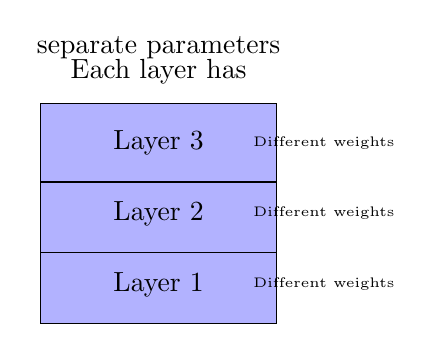
\begin{tikzpicture}[scale=0.6]
    \foreach \y/\label in {0/Layer 1, 1.5/Layer 2, 3/Layer 3} {
        \node[rectangle,draw,fill=blue!30,minimum width=3cm,minimum height=1cm] at (0, \y) {\label};
        \node at (3.5, \y) {\tiny Different weights};
    }

    \node at (0, 4.5) {Each layer has};
    \node at (0, 5) {separate parameters};
\end{tikzpicture}
\end{center}

\vspace{0.5em}

\textbf{Parameters:}
\begin{itemize}\setlength{\itemsep}{0pt}
    \item 12 × (Attention + FFN)
    \item Total: $\sim$110M params
\end{itemize}
\end{column}

\begin{column}{0.48\textwidth}
\textbf{ALBERT (Sharing):}

\begin{center}
\begin{tikzpicture}[scale=0.6]
    \node[rectangle,draw,fill=green!30,minimum width=3cm,minimum height=1cm,align=center] (shared) at (3, 1.5) {Shared\\Parameters};

    \foreach \y/\label in {0/Layer 1, 1.5/Layer 2, 3/Layer 3} {
        \node[rectangle,draw,fill=orange!30,minimum width=2cm,minimum height=1cm] (layer\y) at (0, \y) {\label};
        \draw[->, thick] (shared) -- (layer\y);
    }

    \node at (1.5, 4.5) {All layers use};
    \node at (1.5, 5) {same parameters};
\end{tikzpicture}
\end{center}

\vspace{0.5em}

\textbf{Parameters:}
\begin{itemize}\setlength{\itemsep}{0pt}
    \item 1 × (Attention + FFN)
    \item Total: $\sim$12M params
\end{itemize}
\end{column}
\end{columns}

\vspace{1em}

\textbf{Questions:}
\begin{itemize}\setlength{\itemsep}{0pt}
    \item Does this hurt performance? \alert{Sometimes slightly, but often comparable!}
    \item What's the intuition? Layers learn similar transformations
    \item Trade-off: Memory vs. expressiveness
\end{itemize}
\end{frame}

% ============================================================
% DISTILBERT
% ============================================================
\begin{frame}[shrink=10]{DistilBERT: Knowledge Distillation ⚡}
\textbf{Key idea: Train small model to mimic large model}

\vspace{1em}

\textbf{Knowledge Distillation Process (Sanh et al. 2019):}

\begin{enumerate}\setlength{\itemsep}{0pt}
    \item \textbf{Teacher Model:} Large, pre-trained BERT
    \item \textbf{Student Model:} Smaller model (6 layers instead of 12)
    \item \textbf{Training Objective:}
    \begin{itemize}\setlength{\itemsep}{0pt}
        \item Student learns to match teacher's output distributions
        \item Not just hard labels, but soft probabilities
        \item Also uses MLM loss on original task
    \end{itemize}
\end{enumerate}

\vspace{1em}

\begin{center}
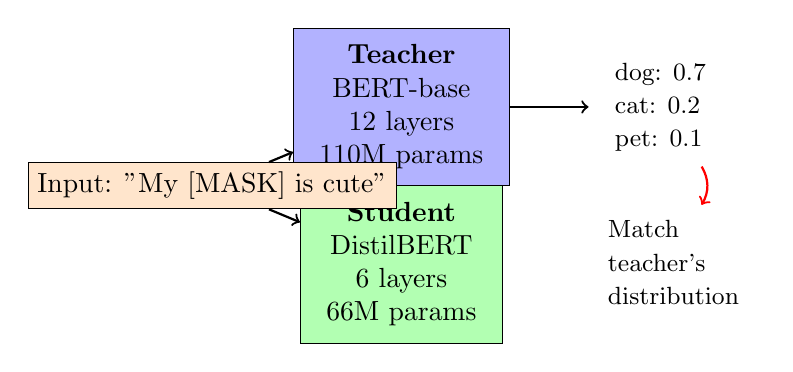
\begin{tikzpicture}[scale=0.8]
    % Teacher
    \node[rectangle,draw,fill=blue!30,minimum width=2.5cm,minimum height=2cm] (teacher) at (0, 2) {
        \begin{tabular}{c}
        \textbf{Teacher} \\
        BERT-base \\
        12 layers \\
        110M params
        \end{tabular}
    };

    % Student
    \node[rectangle,draw,fill=green!30,minimum width=2.5cm,minimum height=2cm] (student) at (0, -0.5) {
        \begin{tabular}{c}
        \textbf{Student} \\
        DistilBERT \\
        6 layers \\
        66M params
        \end{tabular}
    };

    % Input
    \node[rectangle,draw,fill=orange!20] (input) at (-3, 0.75) {Input: "My [MASK] is cute"};

    % Arrows
    \draw[->, thick] (input) -- (teacher);
    \draw[->, thick] (input) -- (student);

    % Output
    \node[right=1cm of teacher] (tout) {
        \begin{tabular}{l}
        \small dog: 0.7 \\
        \small cat: 0.2 \\
        \small pet: 0.1
        \end{tabular}
    };

    \node[right=1cm of student] (sout) {
        \begin{tabular}{l}
        \small Match \\
        \small teacher's \\
        \small distribution
        \end{tabular}
    };

    \draw[->, thick] (teacher) -- (tout);
    \draw[->, thick, red] (tout) to[bend left=30] (sout);
\end{tikzpicture}
\end{center}

\small
\textit{Reference: Sanh et al. (2019) - "DistilBERT, a distilled version of BERT"}
\end{frame}

% ============================================================
% DISTILBERT RESULTS
% ============================================================
\begin{frame}{DistilBERT Results 📊}
\textbf{Significant efficiency gains!}

\vspace{1em}

\begin{center}
\begin{tabular}{lccc}
\toprule
\textbf{Metric} & \textbf{BERT-base} & \textbf{DistilBERT} & \textbf{Ratio} \\
\midrule
Parameters & 110M & 66M & \textbf{40\% smaller} \\
Inference Speed & 1x & 1.6x & \textbf{60\% faster} \\
GLUE Score & 79.6 & 77.0 & \textbf{97\% retained} \\
\bottomrule
\end{tabular}
\end{center}

\vspace{1em}

\textbf{Performance on Specific Tasks:}
\begin{center}
\small
\begin{tabular}{lcc}
\toprule
\textbf{Task} & \textbf{BERT} & \textbf{DistilBERT} \\
\midrule
SQuAD 1.1 (F1) & 90.9 & 86.9 \\
SST-2 (Acc) & 94.9 & 92.7 \\
MNLI (Acc) & 86.7 & 82.2 \\
\bottomrule
\end{tabular}
\end{center}

\vspace{1em}

\textbf{When to Use DistilBERT:}
\begin{itemize}\setlength{\itemsep}{0pt}
    \item Production deployment (latency-critical)
    \item Edge devices (limited memory)
    \item High-throughput scenarios
    \item When 2-3\% performance drop is acceptable
\end{itemize}
\end{frame}

% ============================================================
% ELECTRA
% ============================================================
\begin{frame}[shrink=5]{ELECTRA: Efficient Learning 🔌}
\textbf{Key idea: Learn from all tokens, not just 15\%}

\vspace{1em}

\textbf{ELECTRA's Approach (Clark et al. 2020):}

\begin{itemize}\setlength{\itemsep}{0pt}
    \item \textbf{Replace Token Detection} instead of Masked LM
    \item Use a small generator to replace some tokens
    \item Discriminator learns to detect which tokens were replaced
    \item \alert{Every token provides a training signal!}
\end{itemize}

\vspace{1em}

\begin{center}
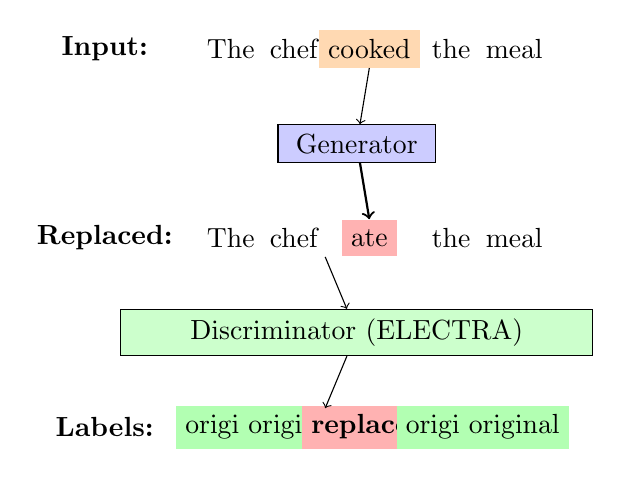
\begin{tikzpicture}[scale=0.8]
    % Input
    \node at (0, 4) {\textbf{Input:}};
    \node at (2, 4) {The};
    \node at (3, 4) {chef};
    \node[fill=orange!30] at (4.2, 4) {cooked};
    \node at (5.5, 4) {the};
    \node at (6.5, 4) {meal};

    % Generator
    \node[rectangle,draw,fill=blue!20,minimum width=2cm] (gen) at (4, 2.5) {Generator};
    \draw[->] (4.2, 3.7) -- (gen);

    % Replaced
    \node at (0, 1) {\textbf{Replaced:}};
    \node at (2, 1) {The};
    \node at (3, 1) {chef};
    \node[fill=red!30] at (4.2, 1) {ate};
    \node at (5.5, 1) {the};
    \node at (6.5, 1) {meal};

    \draw[->, thick] (gen) -- (4.2, 1.3);

    % Discriminator
    \node[rectangle,draw,fill=green!20,minimum width=6cm] (disc) at (4, -0.5) {Discriminator (ELECTRA)};
    \draw[->] (3.5, 0.7) -- (disc);

    % Labels
    \node at (0, -2) {\textbf{Labels:}};
    \node[fill=green!30] at (2, -2) {original};
    \node[fill=green!30] at (3, -2) {original};
    \node[fill=red!30] at (4.2, -2) {\textbf{replaced}};
    \node[fill=green!30] at (5.5, -2) {original};
    \node[fill=green!30] at (6.5, -2) {original};

    \draw[->] (disc) -- (3.5, -1.7);
\end{tikzpicture}
\end{center}

\small
\textit{Reference: Clark et al. (2020) - "ELECTRA: Pre-training Text Encoders as Discriminators"}
\end{frame}

% ============================================================
% ELECTRA BENEFITS
% ============================================================
\begin{frame}[shrink=10]{ELECTRA Benefits ⚡}
\small
\textbf{More efficient pre-training}

\vspace{1em}

\textbf{Advantages:}
\begin{enumerate}\setlength{\itemsep}{0pt}
    \item \textbf{Sample Efficiency}
    \begin{itemize}\setlength{\itemsep}{0pt}
        \item Learn from all tokens (100\%) vs only masked (15\%)
        \item Reaches same performance with less data
        \item Faster convergence
    \end{itemize}

    \vspace{0.5em}

    \item \textbf{Better Performance}
    \begin{itemize}\setlength{\itemsep}{0pt}
        \item ELECTRA-Small outperforms BERT-Small
        \item ELECTRA-Base competitive with BERT-Large
        \item With same compute, ELECTRA is better
    \end{itemize}

    \vspace{0.5em}

    \item \textbf{Computational Efficiency}
    \begin{itemize}\setlength{\itemsep}{0pt}
        \item Smaller generator (1/4 to 1/2 size of discriminator)
        \item Faster to train than BERT
        \item Lower computational cost for same quality
    \end{itemize}
\end{enumerate}

\vspace{1em}

\begin{block}{Key Insight}
Replace Token Detection is more sample-efficient than Masked LM because it provides a learning signal for every token!
\end{block}
\end{frame}

% ============================================================
% COMPARISON TABLE
% ============================================================
\begin{frame}{BERT Variants Comparison 📊}
\textbf{Summary of key variants}

\vspace{1em}

\begin{center}
\tiny
\begin{tabular}{lp{3cm}p{3cm}p{3cm}}
\toprule
\textbf{Model} & \textbf{Key Innovation} & \textbf{Advantages} & \textbf{Best For} \\
\midrule
\textbf{BERT} &
Masked Language Model, bidirectional &
Original, well-studied, strong baseline &
General understanding tasks \\
\midrule
\textbf{RoBERTa} &
Better training (dynamic masking, no NSP, more data) &
Best performance, robust &
When quality matters most \\
\midrule
\textbf{ALBERT} &
Parameter sharing, factorized embeddings &
Fewer parameters, memory efficient &
Limited memory/storage \\
\midrule
\textbf{DistilBERT} &
Knowledge distillation &
Fast inference, small size &
Production, edge deployment \\
\midrule
\textbf{ELECTRA} &
Replace token detection &
Sample efficient, good performance &
Limited pre-training compute \\
\bottomrule
\end{tabular}
\end{center}

\vspace{1em}

\textbf{General Guidelines:}
\begin{itemize}\setlength{\itemsep}{0pt}
    \item \textbf{Best quality:} RoBERTa-Large
    \item \textbf{Best efficiency:} DistilBERT
    \item \textbf{Limited memory:} ALBERT
    \item \textbf{Limited training budget:} ELECTRA
    \item \textbf{Good default:} RoBERTa-Base or BERT-Base
\end{itemize}
\end{frame}

% ============================================================
% OTHER VARIANTS
% ============================================================
\begin{frame}[shrink=10]{Other Notable BERT Variants 🌟}
\textbf{The BERT family keeps growing!}

\vspace{1em}

\begin{enumerate}\setlength{\itemsep}{0pt}
    \item \textbf{DeBERTa (Microsoft, 2020)}
    \begin{itemize}\setlength{\itemsep}{0pt}
        \item Disentangled attention (separate content and position)
        \item Enhanced mask decoder
        \item State-of-the-art on SuperGLUE
    \end{itemize}

    \vspace{0.5em}

    \item \textbf{ERNIE (Baidu, 2019)}
    \begin{itemize}\setlength{\itemsep}{0pt}
        \item Entity-level and phrase-level masking
        \item Knowledge enhancement
        \item Strong on Chinese NLP tasks
    \end{itemize}

    \vspace{0.5em}

    \item \textbf{SpanBERT (Facebook, 2019)}
    \begin{itemize}\setlength{\itemsep}{0pt}
        \item Mask random spans instead of random tokens
        \item Span boundary objective
        \item Better for span-based tasks (QA, coreference)
    \end{itemize}

    \vspace{0.5em}

    \item \textbf{BART (Facebook, 2019)}
    \begin{itemize}\setlength{\itemsep}{0pt}
        \item Encoder-decoder (not encoder-only)
        \item Denoising autoencoder with various corruptions
        \item Excellent for generation tasks
    \end{itemize}
\end{enumerate}
\end{frame}

% ============================================================
% MODEL SELECTION
% ============================================================
\begin{frame}[shrink=5]{Model Selection Guide 🎯}
\textbf{How to choose the right model for your task}

\vspace{1em}

\begin{center}
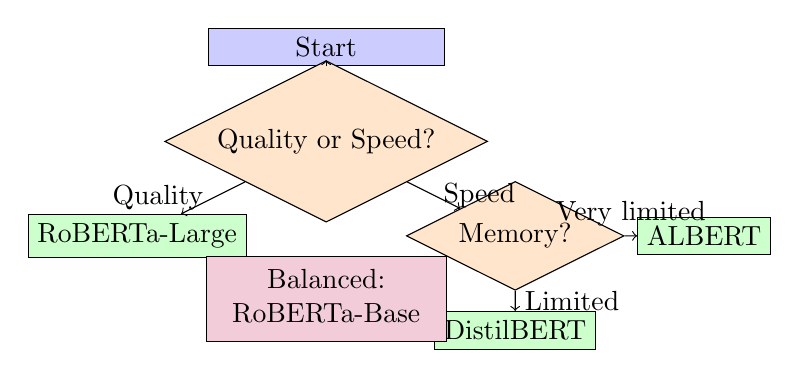
\begin{tikzpicture}[scale=0.8]
    % Start
    \node[rectangle,draw,fill=blue!20,minimum width=3cm] (start) at (0, 4) {Start};

    % Quality vs Speed
    \node[diamond,draw,fill=orange!20,aspect=2,minimum width=2.5cm] (q1) at (0, 2.5) {Quality or Speed?};
    \draw[->] (start) -- (q1);

    % Quality path
    \node[rectangle,draw,fill=green!20] (quality) at (-3, 1) {RoBERTa-Large};
    \draw[->] (q1) -- (quality) node[midway,left] {Quality};

    % Speed path
    \node[diamond,draw,fill=orange!20,aspect=2,minimum width=2cm] (q2) at (3, 1) {Memory?};
    \draw[->] (q1) -- (q2) node[midway,right] {Speed};

    % Speed options
    \node[rectangle,draw,fill=green!20] (distil) at (3, -0.5) {DistilBERT};
    \draw[->] (q2) -- (distil) node[midway,right] {Limited};

    \node[rectangle,draw,fill=green!20] (albert) at (6, 1) {ALBERT};
    \draw[->] (q2) -- (albert) node[midway,above] {Very limited};

    % Balanced
    \node[rectangle,draw,fill=purple!20] (balanced) at (0, 0) {
        \begin{tabular}{c}
        Balanced: \\
        RoBERTa-Base
        \end{tabular}
    };
\end{tikzpicture}
\end{center}

\vspace{1em}

\textbf{Additional Considerations:}
\begin{itemize}\setlength{\itemsep}{0pt}
    \item \textbf{Domain:} Consider domain-specific pre-trained models (BioBERT, SciBERT, etc.)
    \item \textbf{Language:} Multilingual? Use mBERT, XLM-R
    \item \textbf{Task type:} Generation? Consider BART/T5 instead
\end{itemize}
\end{frame}

% ============================================================
% CODE EXAMPLE
% ============================================================
\begin{frame}[fragile]{Using Different BERT Variants 💻}
\textbf{Easy switching with HuggingFace}

\begin{lstlisting}[language=Python]
from transformers import AutoModel, AutoTokenizer

# BERT
bert_model = AutoModel.from_pretrained("bert-base-uncased")
bert_tokenizer = AutoTokenizer.from_pretrained("bert-base-uncased")

# RoBERTa
roberta_model = AutoModel.from_pretrained("roberta-base")
roberta_tokenizer = AutoTokenizer.from_pretrained("roberta-base")

# ALBERT
albert_model = AutoModel.from_pretrained("albert-base-v2")
albert_tokenizer = AutoTokenizer.from_pretrained("albert-base-v2")

# DistilBERT
distilbert_model = AutoModel.from_pretrained("distilbert-base-uncased")
distilbert_tokenizer = AutoTokenizer.from_pretrained("distilbert-base-uncased")

# ELECTRA
electra_model = AutoModel.from_pretrained("google/electra-base-discriminator")
electra_tokenizer = AutoTokenizer.from_pretrained("google/electra-base-discriminator")

# All have the same API!
inputs = tokenizer("Hello, my dog is cute", return_tensors="pt")
outputs = model(**inputs)
\end{lstlisting}
\end{frame}

% ============================================================
% DISCUSSION
% ============================================================
\begin{frame}[shrink=10]{Discussion Questions 💭}
\begin{enumerate}\setlength{\itemsep}{0pt}
    \item \textbf{Training vs Architecture:}
    \begin{itemize}\setlength{\itemsep}{0pt}
        \item RoBERTa shows training matters. Is architecture overrated?
        \item How much can we improve with just better training?
        \item What's the right balance?
    \end{itemize}

    \vspace{0.5em}

    \item \textbf{Parameter Efficiency:}
    \begin{itemize}\setlength{\itemsep}{0pt}
        \item ALBERT shares all layers. Why does this work?
        \item What are the limits of parameter sharing?
        \item Is there a "sweet spot"?
    \end{itemize}

    \vspace{0.5em}

    \item \textbf{Knowledge Distillation:}
    \begin{itemize}\setlength{\itemsep}{0pt}
        \item Why does student learn better from teacher than from labels?
        \item What information is in the soft probabilities?
        \item Can we distill even further?
    \end{itemize}

    \vspace{0.5em}

    \item \textbf{Model Selection:}
    \begin{itemize}\setlength{\itemsep}{0pt}
        \item How do you decide which model to use?
        \item Is it worth fine-tuning multiple variants?
        \item What about model ensembles?
    \end{itemize}
\end{enumerate}
\end{frame}

% ============================================================
% LOOKING AHEAD
% ============================================================
\begin{frame}[shrink=10]{Looking Ahead 🔮}
\textbf{Today we learned:}
\begin{itemize}\setlength{\itemsep}{0pt}
    \item RoBERTa: Better training matters
    \item ALBERT: Parameter sharing for efficiency
    \item DistilBERT: Knowledge distillation
    \item ELECTRA: Replace token detection
    \item How to choose the right variant
\end{itemize}

\vspace{1em}

\textbf{Next lecture (Lecture 17 - Applications of Encoder Models):}
\begin{itemize}\setlength{\itemsep}{0pt}
    \item \alert{Real-world BERT applications}
    \item \alert{Classification, NER, QA, and more}
    \item \alert{Cognitive neuroscience connections}
    \item \alert{Understanding vs pattern matching debate}
    \item \alert{Limitations and future directions}
    \item \alert{Practical deployment tips}
\end{itemize}

\vspace{1em}

\begin{center}
\Large
\textbf{From theory to practice! 🚀}
\end{center}
\end{frame}

% ============================================================
% SUMMARY
% ============================================================
\begin{frame}[shrink=10]{Summary 🎯}
\textbf{Key Takeaways:}

\vspace{1em}

\begin{enumerate}\setlength{\itemsep}{0pt}
    \item \textbf{RoBERTa}
    \begin{itemize}\setlength{\itemsep}{0pt}
        \item Training procedure matters as much as architecture
        \item Remove NSP, dynamic masking, more data = better results
    \end{itemize}

    \item \textbf{ALBERT}
    \begin{itemize}\setlength{\itemsep}{0pt}
        \item Parameter sharing dramatically reduces model size
        \item Factorized embeddings for efficiency
        \item 89\% fewer parameters than BERT
    \end{itemize}

    \item \textbf{DistilBERT}
    \begin{itemize}\setlength{\itemsep}{0pt}
        \item Knowledge distillation for deployment
        \item 40\% smaller, 60\% faster, 97\% performance
    \end{itemize}

    \item \textbf{ELECTRA}
    \begin{itemize}\setlength{\itemsep}{0pt}
        \item Replace token detection more sample-efficient
        \item Learn from all tokens, not just 15\%
    \end{itemize}

    \item \textbf{Model Selection}
    \begin{itemize}\setlength{\itemsep}{0pt}
        \item Choose based on constraints (quality, speed, memory)
        \item HuggingFace makes it easy to experiment
    \end{itemize}
\end{enumerate}
\end{frame}

% ============================================================
% REFERENCES
% ============================================================
\begin{frame}[shrink=10]{References 📚}
\textbf{Essential Papers:}

\vspace{0.5em}

\begin{itemize}\setlength{\itemsep}{0pt}
    \item \textbf{Liu et al. (2019)} - "RoBERTa: A Robustly Optimized BERT Pretraining Approach"
    \item \textbf{Lan et al. (2019)} - "ALBERT: A Lite BERT for Self-supervised Learning"
    \item \textbf{Sanh et al. (2019)} - "DistilBERT, a distilled version of BERT"
    \item \textbf{Clark et al. (2020)} - "ELECTRA: Pre-training Text Encoders as Discriminators"
    \item \textbf{He et al. (2020)} - "DeBERTa: Decoding-enhanced BERT with Disentangled Attention"
\end{itemize}

\vspace{0.5em}

\textbf{Resources:}
\begin{itemize}\setlength{\itemsep}{0pt}
    \item HuggingFace Model Hub: \url{https://huggingface.co/models}
    \item Papers With Code: BERT variants leaderboard
    \item Model Cards: Detailed documentation for each variant
\end{itemize}
\end{frame}

% ============================================================
% QUESTIONS
% ============================================================
\begin{frame}{Questions? 🙋}
\begin{center}
\LARGE
\textbf{Discussion Time}
\end{center}

\vspace{1em}

\textbf{Topics for discussion:}
\begin{itemize}\setlength{\itemsep}{0pt}
    \item BERT variants and improvements
    \item Model selection strategies
    \item Knowledge distillation
    \item Parameter efficiency
    \item Implementation questions
\end{itemize}

\vspace{1em}

\begin{center}
\Large
Thank you! 🙏

\vspace{1em}

Next: Applications and Real-World Use Cases!
\end{center}
\end{frame}

\end{document}
